% sections_3_5.tex : Section 3 (Simulation studies), Section 4 (Application) and
% Section 5 (Discussion) for the LRC-BART revision (Phase 5c, 2026-09-09; humanized
% and shortened after critic/grader round 1). Standalone body: \input after
% sections_1_2.tex. Tables are generated by 05-writing/make_tables.R into
% 05-writing/tables/ and \input here; the Sc4 figure by 05-writing/make_fig_sc4.R;
% application figures from 04-application/. Every number quoted in the text is in
% tables/quoted_numbers.txt or in 04-application/application_report.md.

%==============================================================================
\section{Simulation studies}
\label{sec:sim}
%==============================================================================

\subsection{Design}
\label{sec:sim_design}

Each replicate consists of an RCT of $N=300$ subjects and an external source of $n_2=300$ RWD controls, with $p=10$ covariates $X_j\sim\Normal(\mu_j,1)$, $\bm\mu=(1,-1,0.5,-1,2,-2,2,-3,1,0)$, and $X_1$ replaced with probability $0.15$ by a draw from $\Normal(\pm3,0.5^2)$ so that the sources overlap imperfectly. The RCT randomizes $2{:}1$ for Gaussian outcomes, giving about $n_1=100$ controls, and $3{:}1$ for survival outcomes, giving about $75$, as in a hybrid design with a smaller control arm. The RCT control and RWD outcome surfaces are the same nonlinear function
\begin{equation}
\begin{aligned}
f_0(\bm W)={}&\alpha+\beta_1W_1^2+\beta_2e^{-(W_2+1)^2/2}+\beta_3|W_3-0.5|+\beta_4|W_4+1|\\
&+\beta_5\tanh(W_5-2)+\beta_6\tanh(W_6+2)+2\{b(W_5-2)+b(W_6+2)\}+\textstyle\sum_{j=7}^{10}\beta_jW_j,
\end{aligned}
\label{eq:dgp}
\end{equation}
with $b(u)=u^2/\{1+(u/1.5)^2\}$ and
\[
\bm\beta=(-0.50,-0.75,-0.50,-0.50,-1.35,-0.80,-0.01,-0.01,-0.01,-0.01),
\]
and $\bm W=\bm X$ except where stated; the treated RCT subjects add $\delta=1$ for Gaussian outcomes and $\delta=\log1.4$ on the log-time scale for survival outcomes. Residual standard deviations are $\sigma_1=1.5$ and $\sigma_2=1.8$ for Gaussian outcomes and $1.4$ and $1.8$ for survival outcomes, where the survival time is log-normal, dropout is Exponential$(0.02)$, entry is Uniform$(0,1)$ and administrative censoring occurs at calendar time $3$.

We consider five patterns of agreement between sources. Sc1 assigns the source at random. Sc2 assigns it through $P(D=1\given\bm X)=\logit^{-1}\{(\ell-q_{0.5}(\ell))/0.5\}$ with $\ell=-1.20(X_5+X_6)$, so that source membership depends on the two covariates with the largest outcome effects. Sc3 drives the same assignment by unmeasured $(U_1,U_2)$ that also replace $(X_5,X_6)$ in the outcome, with the observed $(X_5,X_6)$ correlated with $\bm U$ at $\rho\in\{-0.5,0,0.5\}$, so the RWD surface differs from the RCT surface everywhere in a way the covariates cannot remove; Web Appendix~G lists the intercepts and the assignment constants.

Sc4 and Sc5 evaluate borrowing under regional and global outcome shifts. Sc4 keeps the assignment of Sc1 and raises the RWD surface by $\delta_2$ outside a compatible region $\mathcal R=\{X_5>2\}$, so that the true discrepancy $g=f_1-f$ is $-\delta_2$ there and $0$ inside. The region holds half of the RCT population and lies on the covariate with the dominant nonlinear effect, so the shift has to be separated from a slope that $f$ already models. We take $\delta_2\in\{0.5,1,2\}$, one third to $1.3$ RCT residual standard deviations, chosen around the leaf resolution $d_{1/2}$ of Theorem~\ref{thm:map}(a), which at $\sigma_1=1.5$, fifty RCT controls per leaf and the spike scale calibrated in Sc1 is about $0.5$. Sc5 raises the RWD surface by $\delta_2\in\{1,2\}$ everywhere, so the compatible region is empty and borrowing should be suppressed throughout the covariate space. Survival outcomes use Sc4 with $\delta_2\in\{0.5,1\}$ on the log scale and Sc5 with $\delta_2=1$.

The estimands are those of Section~\ref{sec:setting}, standardized to the replicate's RCT profiles: the ATE for Gaussian outcomes, and for survival outcomes the ratio of standardized population medians, whose true value is $1.4$, and the ratio of standardized restricted mean survival times at $t^\ast=3$. Over $R=500$ replicates we report the bias of the posterior mean, the mean posterior SD, the Monte Carlo RMSE of the posterior mean, the coverage of the central 95\% credible interval, and power, the fraction of replicates whose 95\% interval excludes the null value, $0$ for the ATE and $1$ for the ratios; the arm-specific means are summarized the same way. Monte Carlo standard errors are about $0.009$ for a Gaussian ATE bias and $0.01$ for a coverage or power, and the replicate data are paired across methods and scenarios, so paired standard errors of a contrast between two methods are much smaller. For Sc4 and Sc5 we add the RMSE of the posterior mean control surface over all $N$ RCT profiles inside and outside $\mathcal R$, the mean of the borrowing map $\mathcal B_c(x)$ over the RCT control profiles in each region at $c=0.5$ on the outcome scale, and the mean of the posterior mean of $g(x)$ in each region, whose true values are $0$ in $\mathcal R$ and $-\delta_2$ outside it. For every LRC-BART fit we also record the prior $\mathrm{ESS}_0$, the realized ESS, the ceiling, and whether the target was capped. Since $\mathrm{ESS}_0$ averages $\sigma_1^2/\{V^{(b)}+c_gH_g\tau_0^2\}$ over the Stage-1 blocks while the ceiling uses the whole-chain variance, Jensen's inequality puts the printed $\mathrm{ESS}_0$ of a capped fit a few percent above the printed ceiling.

We compare LRC-BART with Bayesian linear and log-normal AFT regressions fitted to the RCT controls alone (LM-NP, AFT-NP), to the pooled controls (LM-CP, AFT-CP) and to the pooled controls with the source indicator as a covariate (LM-PP, AFT-PP); standard BART and AFT-BART \citep{Chipman2010BART,Sparapani2021BART} in the same three configurations (BART-NP, BART-CP, BART-PP), the last being the implicit borrowing of \citet{ZhouJi2021}; the propensity-score composite likelihood PSCL of \citet{Chen2020PSCL}; the MAP prior for the control mean without covariate adjustment; hierarchical linear and AFT models (HierLM, HierAFT); and the two nested versions of the proposed model, C-BART ($w=1$) and the free-offset LRC-BART ($w=0$) of Section~\ref{sec:model}. Web Appendix~G.2 gives their priors, samplers and implementation details.
We also transfer the analysis component of CAHB \citep{Jin2023CAHB} to Sc1, Sc4 and Sc5 in $R=200$ Gaussian replicates paired with the first $200$ full-study replicates. Our choices for the historical smoother, covariate selection, bandwidth, precision scales and joint draws are described in Web Appendix~G.2, together with the ten-covariate and literal-constant variants.

LRC-BART is fitted as in Section~\ref{sec:model}, with $H_f=50$, $H_g=5$, $(\alpha_g,\beta_g)=(0.5,3)$, the range-rule slab, $\nu_0=3$, $w\sim\mathrm{Beta}(1,1)$, and a treated-arm BART with $50$ trees. In Stage 1, we fit the calibration model to the RWD with $1{,}000$ retained draws cut into $B=20$ blocks, take $\sigma_1^2$ from a plain BART fitted to the RCT controls, compute $c_g$ once by Monte Carlo under the $g$-tree prior, and search a geometric grid of $141$ spike scales from $10^{-6}$ to $10$. We report an absolute ladder $N_{\rm target}\in\{50,75,100\}$, with the ceiling override applied when the requested target reaches it, and a fractional ladder at $0.25$, $0.5$ and $0.9$ of the ceiling, with LRC-BART ($100$) as the reference configuration and LRC-BART ($0.9$) as the fractional reference; LRC-BART ($H_g=10$) doubles the discrepancy ensemble. Averaged over scenarios and replicates in the full study, run on $16$ forked workers, a full LRC-BART fit with calibration and treated arm took $2.3$ seconds for Gaussian and $2.5$ seconds for survival outcomes, against $1.6$ and $2.1$ seconds for BART-PP and $1.1$ and $1.6$ for BART-NP, and the whole study ran in $5.6$ hours. The configuration of $g$ was chosen on a development run of $R=200$ paired with the first $200$ replicates here (Web Appendix~G.3).

\subsection{Gaussian outcomes}
\label{sec:sim_gauss}

Table~\ref{tab:gauss} reports the two-arm Gaussian results for selected scenarios and methods, and Web Table~S1 the full set.

Under agreement between sources (Sc1), the RMSE of LRC-BART ($100$) is $0.172$ against $0.205$ for BART-PP and $0.220$ for BART-NP, with coverage $0.94$; the paired difference in mean squared error from BART-PP is $-0.012$ with standard error $0.001$. BART-CP has RMSE $0.142$, followed by C-BART at $0.150$, LRC-BART at $0.172$ and BART-PP at $0.205$. LRC-BART ($100$) has mean prior $\mathrm{ESS}_0$ of $82$, ceiling $127$ and realized ESS $53$, using posterior indicators and $\tau_0^2$. The target exceeds the ceiling in $20\%$ of replicates, triggering the smallest-scale override. Tree-model power is $1.00$ at $\delta=1$, also with a 90\% interval (Web Appendix~G).

Under measured confounding (Sc2), the covariate-adjusted methods have small biases: LRC-BART ($100$) with bias $0.023$ and RMSE $0.192$ against $0.007$ and $0.204$ for BART-PP, whereas BART-CP, which pools the sources, and C-BART, which has a common discrepancy scale without a slab, carry biases of $0.058$ and $0.042$ with coverage $0.91$. The ESS ceiling is substantially lower in Sc2, consistent with the covariate-overlap calculation in Theorem~\ref{thm:ess}(d): the RCT profiles concentrate in regions with limited RWD support, the ceiling falls from $127$ in Sc1 to $23$, every absolute target is capped in every replicate and the three absolute targets give the same fit (Web Table~S3), whereas the fractional ladder still spans prior ESS $5$, $10$ and $16$ with biases $0.012$, $0.016$ and $0.019$. We therefore recommend reporting fractional targets when covariate overlap is poor.

Under unmeasured confounding, Sc3, the RWD surface differs from the RCT surface everywhere by an amount the covariates cannot explain, and the two tree models with fixed commensurate components have substantial bias, as do their linear counterparts: BART-CP has bias $0.98$ at $\rho=0$ with coverage $0$, and C-BART, with one commensurability scale and no slab, has bias $0.23$ with coverage $0.87$, consistent with the unbounded influence under fixed components in Theorem~\ref{thm:influence}.

LRC-BART ($100$) largely suppresses borrowing. Its realized ESS is $1.6$, its map averages $0.07$, and its bias is $0.041$ with coverage $0.94$ and RMSE $0.280$, against $0.029$ and $0.273$ for BART-PP and $-0.002$ and $0.289$ for BART-NP, with similar results at the three values of $\rho$. The $0.04$ residual bias exceeds BART-PP's by $0.012$ (paired Monte Carlo standard error $0.001$). The spike provides a possible explanation: a leaf whose RCT residual mean is not far beyond $d_{1/2}$ keeps a small but nonzero posterior spike probability, and Theorem~\ref{thm:influence} bounds the resulting shift by about one RCT standard error of the leaf. Doubling the discrepancy ensemble raises the bias to $0.055$, as $H_g\tau_0^2$ increases the variation permitted under the spike. This favors a small $H_g$ in this study.

Table~\ref{tab:map} and Figure~\ref{fig:sc4map} report Sc4 and Sc5. At $\delta_2=2$ the map separates the regions: $\bar{\mathcal B}_c$ is $0.64$ over the RCT control profiles in $\mathcal R$ and $0.05$ outside it, and the posterior mean of $g$ averages $-0.26$ in $\mathcal R$ and $-1.71$ outside it against true values of $0$ and $-2$.

Figure~\ref{fig:sc4map} shows how discrepancy estimates vary across the boundary. Away from the boundary at $X_5=2$ the posterior mean of $g$ is $-1.8$ outside $\mathcal R$ and $-0.15$ inside it, short of the truth by about a tenth of the shift on each side, and the map is $0.02$ outside and $0.7$ inside; the transition occupies the unit around the boundary, with $g$ averaging $-1.66$ in the half-unit bin below it and $-0.44$ in the half-unit bin above it. The boundary is learned from the RCT controls alone, about four of them per $0.1$ of $X_5$, and the pooled surface $f$, which is estimated from both sources, smooths the RWD step across it, leaving the shallow discrepancy ensemble $g$ to estimate the remaining difference. The discrepancy underestimation persisted with $f$ fixed at the truth and under every $g$ prior we tried (Web Appendix~G.3), so the configurations examined did not resolve it.

The empirical ATE bias at $\delta_2=2$ is $0.000$ (coverage $0.92$), because the errors on the two sides of the boundary have opposite signs and the estimand averages over both. Control-surface estimation is less accurate: its RMSE over the RCT profiles in $\mathcal R$ is $0.824$ against $0.785$ for BART-PP, and outside $\mathcal R$ it is $0.857$ against $0.822$, so at $\delta_2=2$ LRC-BART does not beat the free-offset model on the surface, while C-BART, at $1.087$ outside $\mathcal R$, has a larger error than either method. A secondary version of Sc4 places the shift on $X_7$, a covariate with negligible effect, and the map and ATE results are similar to those on $X_5$ at both $\delta_2=2$ and $\delta_2=1$ (Web Appendix~G.3).

At $\delta_2=1$, a shift of about twice $d_{1/2}$, the map separates only partially ($0.62$ against $0.52$), the posterior mean of $g$ is $-0.6$ outside $\mathcal R$ and $-0.25$ inside it (Figure~\ref{fig:sc4map}), and LRC-BART borrows too much outside $\mathcal R$: the ATE bias is $-0.041$ (paired difference from BART-PP $-0.039$, standard error $0.003$), the RMSE $0.223$ against $0.207$, and the coverage $0.89$, whereas C-BART and BART-CP have biases of $-0.21$ and $-0.34$.

At $\delta_2=0.5$, below the stated resolution, the map is flat at $0.84$, $g$ averages $-0.15$ in $\mathcal R$ and $-0.18$ outside it, and the bias is $-0.043$ with RMSE $0.200$, below BART-PP's $0.203$ because the variance reduction offsets the bias in this scenario. Lower fractional targets reduce bias under the moderate shift, $-0.032$ at a quarter of the ceiling against $-0.041$, at a cost of $0.01$ in RMSE in Sc1 (Web Table~S3).

Under the global shift of Sc5, LRC-BART suppresses borrowing: at $\delta_2=2$ the map averages $0.01$, the realized ESS is $0.2$, the bias is $-0.001$ and the RMSE $0.203$, against BART-NP's $0.220$ and BART-PP's $0.205$, whereas C-BART and BART-CP have biases of $-0.32$ and $-1.39$; at $\delta_2=1$ the map is $0.10$ and the bias $-0.005$.

The realized regional ESS summarizes learned local precision (Table~\ref{tab:map}). Across the first $200$ replicates, it is $32.7$ and $31.9$ on the two sides of the Sc4 partition under Sc1. Under Sc4 it is $15.1$ in $\mathcal R$ and $12.7$ outside at $\delta_2=1$, and $9.5$ and $0.44$ at $\delta_2=2$. Under Sc5 with $\delta_2=2$, it is about $0.2$ on both sides. These quantities use the control mean standardized within each region and are not additive. The prior pointwise ESS uses the RWD fit and cannot establish that trial outcomes support regional borrowing.

The surface loss persists away from the boundary. On RCT control profiles with $X_5>2.5$, the Sc4 $\delta_2=2$ RMSE is $0.747$ for LRC-BART and $0.723$ for BART-PP, a paired difference of $0.024$ with standard error $0.005$ over $200$ replicates. Using all RCT profiles in $\mathcal R$ over those same replicates gives a difference of $0.039$ with standard error $0.006$. Web Appendix~G.3 reports both profile sets. Thus the evidence for LRC-BART is its efficiency under Sc1 and its regional compatibility and ESS summaries, with a surface-estimation loss under Sc4.

The transferred CAHB analysis has Sc1 RMSE $0.258$, compared with $0.175$ for LRC-BART and $0.223$ for BART-NP over the same $200$ replicates. At Sc4 $\delta_2=2$, its bias is $-0.333$ and its historical precision shares average $0.49$ and $0.41$ in the two regions. At Sc5 $\delta_2=1$, its bias is $-0.437$. These transfer-specific results do not establish a general ranking of CAHB and tree-based borrowing.

\begin{figure}[htbp]
\centering
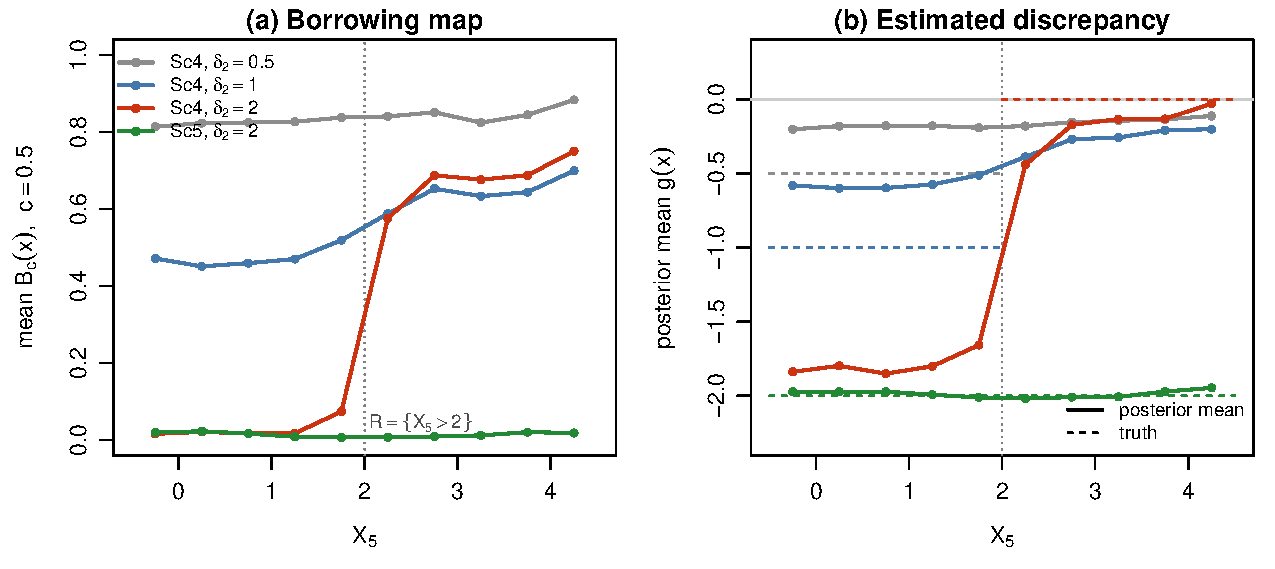
\includegraphics[width=\textwidth]{figures/fig_sc4_map.pdf}
\caption{Regional and global shifts, Gaussian outcomes, LRC-BART ($100$): (a) the borrowing map $\mathcal B_c(x)=P(|g(x)|<0.5\given\text{data})$ and (b) the posterior mean of $g(x)$, both averaged over the RCT control profiles in bins of width $0.5$ on $X_5$ across the first $40$ replicates. The RWD surface is raised by $\delta_2$ where $X_5\le2$ (Sc4) or everywhere (Sc5), so the true discrepancy, dashed in (b), is $-\delta_2$ there.}
\label{fig:sc4map}
\end{figure}

\begingroup
\singlespacing
\scriptsize
\setlength{\tabcolsep}{2.5pt}
\renewcommand{\arraystretch}{1.0}
\begin{longtable}{llccccccc}
\caption{Gaussian outcomes, two-arm design, $R=500$ replicates: average treatment effect (ATE) bias, mean posterior SD, Monte Carlo RMSE, coverage of the 95\% credible interval, and power (95\% interval excludes zero at $\delta=1$), with bias and RMSE of the RCT-standardized control mean. Sc4 raises the RWD control surface by $\delta_2$ outside $\mathcal R=\{X_5>2\}$; Sc5 raises it everywhere. LRC-BART (100) targets a prior ESS of 100 RCT controls and LRC-BART (0.9) targets 0.9 of the ESS ceiling; CAHB uses $R=200$ paired replicates and our transfer described in Web Appendix~G.2; other rows use $R=500$. C-BART is LRC-BART with $w=1$. PSCL reports no arm-specific means. The full table with every scenario and method is Web Table~S1.}\label{tab:gauss}\\
\toprule
& & \multicolumn{5}{c}{ATE} & \multicolumn{2}{c}{Control mean} \\
\cmidrule(lr){3-7}\cmidrule(lr){8-9}
Scenario & Method & Bias & SD & RMSE & Cov & Pow & Bias & RMSE \\
\midrule
\endfirsthead
\multicolumn{9}{l}{\textit{Table \ref{tab:gauss}, continued}}\\
\toprule
& & \multicolumn{5}{c}{ATE} & \multicolumn{2}{c}{Control mean} \\
\cmidrule(lr){3-7}\cmidrule(lr){8-9}
Scenario & Method & Bias & SD & RMSE & Cov & Pow & Bias & RMSE \\
\midrule
\endhead
\midrule
\endfoot
\bottomrule
\endlastfoot
\multirow{11}{*}{Sc1} & LM-PP & $-$0.002 & 0.347 & 0.337 & 0.94 & 0.85 & 0.001 & 0.243 \\*
& BART-NP & 0.004 & 0.203 & 0.220 & 0.91 & 1.00 & 0.001 & 0.185 \\*
& BART-CP & 0.008 & 0.145 & 0.142 & 0.96 & 1.00 & $-$0.003 & 0.096 \\*
& BART-PP & 0.006 & 0.207 & 0.205 & 0.94 & 1.00 & $-$0.001 & 0.170 \\*
& PSCL & 0.005 & 0.269 & 0.261 & 0.95 & 0.97 & $-$0.005 & 0.171 \\*
& MAP (100) & 0.006 & 0.292 & 0.265 & 0.97 & 0.95 & $-$0.005 & 0.174 \\*
& HierLM & $-$0.003 & 0.338 & 0.341 & 0.93 & 0.85 & 0.003 & 0.249 \\*
& C-BART & 0.007 & 0.155 & 0.150 & 0.95 & 1.00 & $-$0.002 & 0.106 \\*
& LRC-BART (100) & 0.009 & 0.171 & 0.172 & 0.94 & 1.00 & $-$0.004 & 0.134 \\*
& LRC-BART (0.9) & 0.011 & 0.171 & 0.171 & 0.95 & 1.00 & $-$0.005 & 0.132 \\*
& CAHB & $-$0.003 & 0.410 & 0.258 & 1.00 & 0.78 & $-$0.023 & 0.184 \\
\midrule
\multirow{10}{*}{Sc2} & LM-PP & 0.010 & 0.340 & 0.331 & 0.95 & 0.84 & $-$0.010 & 0.248 \\*
& BART-NP & $-$0.008 & 0.201 & 0.219 & 0.93 & 1.00 & 0.009 & 0.180 \\*
& BART-CP & 0.058 & 0.177 & 0.195 & 0.91 & 1.00 & $-$0.056 & 0.151 \\*
& BART-PP & 0.007 & 0.208 & 0.204 & 0.96 & 1.00 & $-$0.005 & 0.163 \\*
& PSCL & 0.024 & 0.321 & 0.292 & 0.97 & 0.91 & $-$0.029 & 0.205 \\*
& MAP (100) & 0.332 & 0.360 & 0.491 & 0.83 & 0.97 & $-$0.337 & 0.424 \\*
& HierLM & $-$0.011 & 0.318 & 0.321 & 0.95 & 0.88 & 0.011 & 0.238 \\*
& C-BART & 0.042 & 0.168 & 0.186 & 0.91 & 1.00 & $-$0.041 & 0.141 \\*
& LRC-BART (100) & 0.023 & 0.181 & 0.192 & 0.94 & 1.00 & $-$0.021 & 0.148 \\*
& LRC-BART (0.9) & 0.019 & 0.183 & 0.193 & 0.93 & 1.00 & $-$0.017 & 0.151 \\
\midrule
\multirow{10}{*}{Sc3, $\rho=0$} & LM-PP & 0.043 & 0.356 & 0.346 & 0.95 & 0.85 & $-$0.027 & 0.241 \\*
& BART-NP & $-$0.002 & 0.292 & 0.289 & 0.94 & 0.92 & 0.024 & 0.219 \\*
& BART-CP & 0.984 & 0.202 & 1.003 & 0.00 & 1.00 & $-$0.962 & 0.971 \\*
& BART-PP & 0.029 & 0.275 & 0.273 & 0.94 & 0.96 & $-$0.007 & 0.197 \\*
& PSCL & 0.704 & 0.269 & 0.753 & 0.26 & 1.00 & $-$0.693 & 0.713 \\*
& MAP (100) & 0.363 & 0.360 & 0.504 & 0.82 & 0.97 & $-$0.352 & 0.431 \\*
& HierLM & 0.039 & 0.362 & 0.354 & 0.96 & 0.82 & $-$0.023 & 0.253 \\*
& C-BART & 0.226 & 0.300 & 0.380 & 0.87 & 0.98 & $-$0.204 & 0.311 \\*
& LRC-BART (100) & 0.041 & 0.284 & 0.280 & 0.94 & 0.96 & $-$0.018 & 0.206 \\*
& LRC-BART (0.9) & 0.037 & 0.282 & 0.277 & 0.94 & 0.96 & $-$0.015 & 0.203 \\
\midrule
\multirow{11}{*}{Sc4, $X_5$, $\delta_2=1$} & LM-PP & $-$0.012 & 0.349 & 0.339 & 0.95 & 0.83 & 0.011 & 0.245 \\*
& BART-NP & 0.004 & 0.203 & 0.220 & 0.91 & 1.00 & 0.001 & 0.185 \\*
& BART-CP & $-$0.338 & 0.146 & 0.368 & 0.35 & 1.00 & 0.343 & 0.357 \\*
& BART-PP & $-$0.002 & 0.209 & 0.207 & 0.95 & 1.00 & 0.007 & 0.173 \\*
& PSCL & $-$0.246 & 0.271 & 0.358 & 0.87 & 0.80 & 0.247 & 0.300 \\*
& MAP (100) & $-$0.224 & 0.306 & 0.361 & 0.91 & 0.75 & 0.224 & 0.292 \\*
& HierLM & $-$0.025 & 0.338 & 0.343 & 0.94 & 0.83 & 0.024 & 0.250 \\*
& C-BART & $-$0.207 & 0.173 & 0.273 & 0.73 & 1.00 & 0.212 & 0.258 \\*
& LRC-BART (100) & $-$0.041 & 0.195 & 0.223 & 0.89 & 1.00 & 0.046 & 0.194 \\*
& LRC-BART (0.9) & $-$0.041 & 0.196 & 0.224 & 0.90 & 1.00 & 0.047 & 0.194 \\*
& CAHB & $-$0.208 & 0.413 & 0.333 & 0.98 & 0.42 & 0.181 & 0.262 \\
\midrule
\multirow{11}{*}{Sc4, $X_5$, $\delta_2=2$} & LM-PP & $-$0.023 & 0.354 & 0.343 & 0.95 & 0.81 & 0.022 & 0.249 \\*
& BART-NP & 0.004 & 0.203 & 0.220 & 0.91 & 1.00 & 0.001 & 0.185 \\*
& BART-CP & $-$0.685 & 0.149 & 0.701 & 0.00 & 0.56 & 0.690 & 0.698 \\*
& BART-PP & $-$0.006 & 0.209 & 0.205 & 0.96 & 1.00 & 0.011 & 0.170 \\*
& PSCL & $-$0.498 & 0.273 & 0.562 & 0.54 & 0.44 & 0.498 & 0.528 \\*
& MAP (100) & $-$0.377 & 0.333 & 0.495 & 0.78 & 0.46 & 0.378 & 0.437 \\*
& HierLM & $-$0.044 & 0.339 & 0.345 & 0.94 & 0.81 & 0.043 & 0.253 \\*
& C-BART & $-$0.227 & 0.197 & 0.391 & 0.66 & 0.90 & 0.232 & 0.383 \\*
& LRC-BART (100) & 0.000 & 0.189 & 0.202 & 0.92 & 1.00 & 0.005 & 0.168 \\*
& LRC-BART (0.9) & $-$0.000 & 0.189 & 0.202 & 0.93 & 1.00 & 0.006 & 0.170 \\*
& CAHB & $-$0.333 & 0.422 & 0.453 & 0.95 & 0.25 & 0.309 & 0.398 \\
\midrule
\multirow{11}{*}{Sc5, $\delta_2=2$} & LM-PP & $-$0.042 & 0.347 & 0.339 & 0.94 & 0.80 & 0.042 & 0.246 \\*
& BART-NP & 0.004 & 0.203 & 0.220 & 0.91 & 1.00 & 0.001 & 0.185 \\*
& BART-CP & $-$1.390 & 0.152 & 1.398 & 0.00 & 0.72 & 1.395 & 1.399 \\*
& BART-PP & $-$0.012 & 0.208 & 0.205 & 0.95 & 1.00 & 0.017 & 0.171 \\*
& PSCL & $-$1.002 & 0.269 & 1.035 & 0.04 & 0.04 & 1.002 & 1.017 \\*
& MAP (100) & $-$0.395 & 0.348 & 0.525 & 0.78 & 0.41 & 0.395 & 0.465 \\*
& HierLM & $-$0.038 & 0.338 & 0.344 & 0.94 & 0.82 & 0.037 & 0.251 \\*
& C-BART & $-$0.316 & 0.194 & 0.650 & 0.76 & 0.93 & 0.322 & 0.648 \\*
& LRC-BART (100) & $-$0.001 & 0.190 & 0.203 & 0.92 & 1.00 & 0.005 & 0.171 \\*
& LRC-BART (0.9) & $-$0.001 & 0.190 & 0.205 & 0.92 & 1.00 & 0.006 & 0.171 \\*
& CAHB & $-$0.067 & 0.479 & 0.400 & 0.95 & 0.52 & 0.041 & 0.326 \\
\end{longtable}
\endgroup

\begingroup
\singlespacing
\scriptsize
\setlength{\tabcolsep}{2.5pt}
\renewcommand{\arraystretch}{1.0}
\begin{longtable}{llccccccccc}
\caption{Regional and global shifts, Gaussian outcomes, $R=500$: ATE bias and coverage; RMSE of the posterior mean control surface over all $N$ RCT profiles (treated and control) inside the compatible region $\mathcal R$ and outside it; the borrowing map $\mathcal B_c(x)=P(|g(x)|<0.5\mid\text{data})$ averaged over the RCT control profiles in each region; the posterior mean of $g(x)$ averaged over each region (true value $0$ in $\mathcal R$ and $-\delta_2$ in $\mathcal R^c$); and the realized ESS. In Sc5 the compatible region is empty. Sc4$'$ places the shift on the null covariate $X_7$. LRC-BART ($w=0$) has no spike, so its map reflects the slab alone. CAHB rows use $R=200$; all other rows use $R=500$. CAHB precision shares and effective sizes have different definitions and are reported separately in Web Appendix~G.2. For Sc1, the two columns use the Sc4 partition although both regions are compatible.}\label{tab:map}\\
\toprule
& & \multicolumn{2}{c}{ATE} & \multicolumn{2}{c}{Surface RMSE} & \multicolumn{2}{c}{$\bar{\mathcal B}_c$} & \multicolumn{2}{c}{Mean $\hat g$} & \\
\cmidrule(lr){3-4}\cmidrule(lr){5-6}\cmidrule(lr){7-8}\cmidrule(lr){9-10}
Scenario & Method & Bias & Cov & $\mathcal R$ & $\mathcal R^c$ & $\mathcal R$ & $\mathcal R^c$ & $\mathcal R$ & $\mathcal R^c$ & ESS \\
\midrule
\endfirsthead
\multicolumn{11}{l}{\textit{Table \ref{tab:map}, continued}}\\
\toprule
& & \multicolumn{2}{c}{ATE} & \multicolumn{2}{c}{Surface RMSE} & \multicolumn{2}{c}{$\bar{\mathcal B}_c$} & \multicolumn{2}{c}{Mean $\hat g$} & \\
\cmidrule(lr){3-4}\cmidrule(lr){5-6}\cmidrule(lr){7-8}\cmidrule(lr){9-10}
Scenario & Method & Bias & Cov & $\mathcal R$ & $\mathcal R^c$ & $\mathcal R$ & $\mathcal R^c$ & $\mathcal R$ & $\mathcal R^c$ & ESS \\
\midrule
\endhead
\midrule
\endfoot
\bottomrule
\endlastfoot
\multirow{5}{*}{Sc1} & BART-PP & 0.006 & 0.94 & 0.750 & 0.780 & --- & --- & --- & --- & --- \\*
& C-BART & 0.007 & 0.95 & 0.728 & 0.756 & 1.00 & 1.00 & 0.00 & 0.00 & 81.0 \\*
& LRC-BART ($w=0$) & 0.009 & 0.92 & 0.755 & 0.783 & 0.79 & 0.79 & $-$0.00 & 0.01 & 0.1 \\*
& LRC-BART (100) & 0.009 & 0.94 & 0.736 & 0.763 & 0.92 & 0.92 & $-$0.00 & 0.00 & 52.5 \\*
& CAHB & $-$0.003 & 1.00 & 2.071 & 2.273 & --- & --- & --- & --- & --- \\
\midrule
\multirow{4}{*}{Sc4 (0.5)} & BART-PP & 0.000 & 0.95 & 0.758 & 0.795 & --- & --- & --- & --- & --- \\*
& C-BART & $-$0.109 & 0.90 & 0.736 & 0.799 & 0.98 & 0.98 & $-$0.06 & $-$0.06 & 79.4 \\*
& LRC-BART ($w=0$) & 0.007 & 0.93 & 0.768 & 0.795 & 0.71 & 0.69 & $-$0.21 & $-$0.27 & 0.1 \\*
& LRC-BART (100) & $-$0.043 & 0.92 & 0.751 & 0.796 & 0.84 & 0.83 & $-$0.15 & $-$0.18 & 42.9 \\
\midrule
\multirow{5}{*}{Sc4 (1)} & BART-PP & $-$0.002 & 0.95 & 0.784 & 0.820 & --- & --- & --- & --- & --- \\*
& C-BART & $-$0.207 & 0.73 & 0.749 & 0.915 & 0.91 & 0.90 & $-$0.14 & $-$0.16 & 73.6 \\*
& LRC-BART ($w=0$) & 0.006 & 0.93 & 0.801 & 0.827 & 0.51 & 0.40 & $-$0.35 & $-$0.63 & 0.1 \\*
& LRC-BART (100) & $-$0.041 & 0.89 & 0.783 & 0.843 & 0.62 & 0.52 & $-$0.32 & $-$0.52 & 20.8 \\*
& CAHB & $-$0.208 & 0.98 & 2.133 & 2.207 & --- & --- & --- & --- & --- \\
\midrule
\multirow{5}{*}{Sc4 (2)} & BART-PP & $-$0.006 & 0.96 & 0.785 & 0.822 & --- & --- & --- & --- & --- \\*
& C-BART & $-$0.227 & 0.66 & 0.801 & 1.087 & 0.66 & 0.39 & $-$0.30 & $-$0.97 & 45.7 \\*
& LRC-BART ($w=0$) & 0.004 & 0.92 & 0.836 & 0.858 & 0.57 & 0.05 & $-$0.25 & $-$1.73 & 0.1 \\*
& LRC-BART (100) & 0.000 & 0.92 & 0.824 & 0.857 & 0.64 & 0.05 & $-$0.26 & $-$1.71 & 0.8 \\*
& CAHB & $-$0.333 & 0.95 & 2.172 & 2.157 & --- & --- & --- & --- & --- \\
\midrule
\multirow{4}{*}{Sc4$'$ (1)} & BART-PP & $-$0.001 & 0.96 & 0.807 & 0.810 & --- & --- & --- & --- & --- \\*
& C-BART & $-$0.206 & 0.73 & 0.767 & 0.899 & 0.91 & 0.90 & $-$0.15 & $-$0.16 & 73.3 \\*
& LRC-BART ($w=0$) & 0.009 & 0.92 & 0.820 & 0.817 & 0.52 & 0.41 & $-$0.37 & $-$0.63 & 0.1 \\*
& LRC-BART (100) & $-$0.038 & 0.90 & 0.805 & 0.833 & 0.62 & 0.52 & $-$0.33 & $-$0.52 & 20.5 \\
\midrule
\multirow{4}{*}{Sc4$'$ (2)} & BART-PP & $-$0.002 & 0.95 & 0.805 & 0.806 & --- & --- & --- & --- & --- \\*
& C-BART & $-$0.218 & 0.69 & 0.828 & 1.075 & 0.64 & 0.38 & $-$0.33 & $-$0.97 & 44.7 \\*
& LRC-BART ($w=0$) & 0.007 & 0.92 & 0.859 & 0.848 & 0.57 & 0.05 & $-$0.25 & $-$1.74 & 0.1 \\*
& LRC-BART (100) & 0.001 & 0.93 & 0.850 & 0.848 & 0.64 & 0.05 & $-$0.26 & $-$1.71 & 0.8 \\
\midrule
\multirow{5}{*}{Sc5 (1)} & BART-PP & $-$0.004 & 0.95 & --- & 0.769 & --- & --- & --- & --- & --- \\*
& C-BART & $-$0.244 & 0.68 & --- & 0.821 & --- & 0.43 & --- & $-$0.60 & 41.5 \\*
& LRC-BART ($w=0$) & 0.007 & 0.92 & --- & 0.769 & --- & 0.10 & --- & $-$1.00 & 0.1 \\*
& LRC-BART (100) & $-$0.005 & 0.91 & --- & 0.768 & --- & 0.10 & --- & $-$0.98 & 1.2 \\*
& CAHB & $-$0.437 & 0.91 & --- & 2.203 & --- & --- & --- & --- & --- \\
\midrule
\multirow{5}{*}{Sc5 (2)} & BART-PP & $-$0.012 & 0.95 & --- & 0.771 & --- & --- & --- & --- & --- \\*
& C-BART & $-$0.316 & 0.76 & --- & 0.932 & --- & 0.19 & --- & $-$1.54 & 45.4 \\*
& LRC-BART ($w=0$) & 0.006 & 0.93 & --- & 0.771 & --- & 0.01 & --- & $-$2.00 & 0.1 \\*
& LRC-BART (100) & $-$0.001 & 0.92 & --- & 0.771 & --- & 0.01 & --- & $-$1.99 & 0.2 \\*
& CAHB & $-$0.067 & 0.95 & --- & 1.983 & --- & --- & --- & --- & --- \\
\end{longtable}
\endgroup
\begin{center}\scriptsize
\par\medskip
\begin{tabular}{lcc}
\toprule
Scenario & Regional ESS, $X_5>2$ & Regional ESS, $X_5\le2$ \\
\midrule
Sc1 & 32.66 & 31.86 \\
Sc4 (1) & 15.14 & 12.74 \\
Sc4 (2) & 9.51 & 0.44 \\
Sc5 (2) & 0.24 & 0.24 \\
\bottomrule
\end{tabular}
\par\smallskip\parbox{\textwidth}{\scriptsize Regional realized ESS for LRC-BART (100), averaged over the first 200 paired replicates. Each estimand is the control mean standardized to all RCT profiles in that region. The partition is held fixed for Sc1 and Sc5; both regions are compatible in Sc1 and neither is compatible in Sc5. Regional effective sizes are not additive.}
\end{center}


\subsection{Survival outcomes}
\label{sec:sim_surv}

Table~\ref{tab:surv} reports the survival study for the median ratio and the RMST ratio side by side, and Web Table~S2 the full set. With $75$ RCT controls and about a quarter of the times censored, the median ratio has a wide and skewed posterior under every method, and its posterior mean carries an upward bias that grows with the posterior spread: BART-NP has bias $0.26$ and RMSE $0.51$ in Sc1, where its RMST-ratio bias is $0.13$, and AFT-NP is wider still. Borrowing reduces this uncertainty at the studied sample size.

In Sc1 LRC-BART ($100$) has median-ratio bias $0.045$ and RMSE $0.312$ against $0.032$ and $0.345$ for BART-PP, with power $0.34$ against $0.25$, and its RMST-ratio RMSE is $0.097$ against $0.106$; in Sc2, where the ceiling falls to $40$ and the absolute targets are capped, the two are within $0.03$ of each other on both estimands.

Under unmeasured confounding (Sc3), the tree models with a fixed commensurate component have large biases, as in the Gaussian study: BART-CP with median-ratio bias $2.3$ and C-BART with $0.58$ at $\rho=0$, and LRC-BART abstains with a realized ESS of $2.3$. Its median-ratio bias is then $0.15$ against $0.04$ for BART-PP and $0.19$ for BART-NP, with RMSE $0.558$ against $0.451$ and coverage $0.94$; the paired difference in bias from BART-PP is $0.11$ with standard error $0.005$, the largest loss to BART-PP in the study. The control log-median is biased by only $0.02$, against $-0.006$ for BART-PP, so most of the difference on the ratio scale comes from the wider posterior LRC-BART has once it has switched borrowing off with $75$ controls, with posterior SD $0.52$ against $0.39$, together with the nonlinear transformation to the ratio scale. On the RMST ratio the biases are $0.031$ and $-0.005$ and the RMSEs $0.146$ and $0.137$, a paired difference in mean squared error of $0.003$ with standard error $0.001$. We report both estimands because the median ratio amplifies a small control bias and a wide posterior in a way the RMST ratio does not, and the RMST ratio is the estimand of the application.

Under the regional shift, Sc4 at $\delta_2=1$ on the log scale with a residual SD of $1.4$, the map separates weakly, $0.64$ in $\mathcal R$ against $0.58$ outside, and the treatment-effect biases are $-0.011$ on the median ratio and $-0.037$ on the RMST ratio where C-BART and BART-CP have biases of $-0.20$ and $-0.37$; under the global shift of Sc5 the map is $0.16$, the median-ratio bias $0.03$, and C-BART's $-0.23$. Web Table~S4 gives the map and surface summaries for the survival study, and the fractional ladder behaves as in the Gaussian study.

\begin{table}[htbp]
\centering
\singlespacing
\caption{Survival outcomes, two-arm design, $R=500$: bias, Monte Carlo RMSE, coverage and power (95\% interval excludes one) for the ratio of standardized population medians (true value $1.4$) and the ratio of standardized restricted mean survival times at $t^\ast=3$. Sc4 raises the RWD log-time surface by $\delta_2=1$ outside $\mathcal R=\{X_5>2\}$ and Sc5 by $1$ everywhere. Point estimates are posterior means. The full table is Web Table~S2.}
\label{tab:surv}
\scriptsize
\setlength{\tabcolsep}{4pt}
\renewcommand{\arraystretch}{0.8}
\begin{adjustbox}{max width=\textwidth,max totalheight=0.68\textheight}
\begin{tabular}{llcccccccc}
\toprule
& & \multicolumn{4}{c}{Median ratio} & \multicolumn{4}{c}{RMST ratio, $t^\ast=3$} \\
\cmidrule(lr){3-6}\cmidrule(lr){7-10}
Scenario & Method & Bias & RMSE & Cov & Pow & Bias & RMSE & Cov & Pow \\
\midrule
\multirow{8}{*}{Sc1} & AFT-PP & 0.261 & 0.737 & 0.95 & 0.12 & $-$0.009 & 0.142 & 0.94 & 0.10 \\
& BART-NP & 0.260 & 0.511 & 0.92 & 0.46 & 0.131 & 0.206 & 0.87 & 0.47 \\
& BART-CP & 0.064 & 0.232 & 0.96 & 0.63 & $-$0.011 & 0.072 & 0.95 & 0.35 \\
& BART-PP & 0.032 & 0.345 & 0.95 & 0.25 & $-$0.023 & 0.106 & 0.94 & 0.17 \\
& HierAFT & 0.246 & 0.733 & 0.94 & 0.12 & $-$0.008 & 0.152 & 0.92 & 0.11 \\
& C-BART & 0.034 & 0.248 & 0.97 & 0.42 & 0.003 & 0.079 & 0.95 & 0.32 \\
& LRC-BART (100) & 0.045 & 0.312 & 0.95 & 0.34 & 0.003 & 0.097 & 0.94 & 0.28 \\
& LRC-BART (0.9) & 0.042 & 0.304 & 0.96 & 0.38 & 0.002 & 0.095 & 0.95 & 0.30 \\
\midrule
\multirow{8}{*}{Sc2} & AFT-PP & 0.389 & 0.818 & 0.95 & 0.19 & 0.050 & 0.154 & 0.95 & 0.20 \\
& BART-NP & 0.251 & 0.495 & 0.91 & 0.43 & 0.110 & 0.177 & 0.88 & 0.45 \\
& BART-CP & 0.194 & 0.383 & 0.93 & 0.56 & 0.037 & 0.100 & 0.94 & 0.43 \\
& BART-PP & 0.036 & 0.335 & 0.95 & 0.24 & $-$0.002 & 0.097 & 0.95 & 0.21 \\
& HierAFT & 0.233 & 0.695 & 0.97 & 0.14 & 0.001 & 0.134 & 0.95 & 0.12 \\
& C-BART & 0.138 & 0.331 & 0.93 & 0.55 & 0.043 & 0.104 & 0.92 & 0.49 \\
& LRC-BART (100) & 0.061 & 0.322 & 0.94 & 0.34 & 0.018 & 0.100 & 0.93 & 0.31 \\
& LRC-BART (0.9) & 0.058 & 0.325 & 0.94 & 0.33 & 0.017 & 0.100 & 0.94 & 0.30 \\
\midrule
\multirow{8}{*}{Sc3, $\rho=0$} & AFT-PP & 0.440 & 0.919 & 0.94 & 0.19 & 0.054 & 0.158 & 0.95 & 0.19 \\
& BART-NP & 0.186 & 0.571 & 0.90 & 0.30 & 0.058 & 0.173 & 0.92 & 0.21 \\
& BART-CP & 2.308 & 2.412 & 0.00 & 1.00 & 0.588 & 0.607 & 0.01 & 1.00 \\
& BART-PP & 0.041 & 0.451 & 0.91 & 0.20 & $-$0.005 & 0.137 & 0.92 & 0.15 \\
& HierAFT & 0.337 & 0.890 & 0.95 & 0.13 & 0.006 & 0.147 & 0.95 & 0.11 \\
& C-BART & 0.576 & 0.909 & 0.88 & 0.40 & 0.139 & 0.222 & 0.85 & 0.38 \\
& LRC-BART (100) & 0.155 & 0.558 & 0.94 & 0.17 & 0.031 & 0.146 & 0.94 & 0.18 \\
& LRC-BART (0.9) & 0.148 & 0.554 & 0.94 & 0.17 & 0.029 & 0.144 & 0.93 & 0.18 \\
\midrule
\multirow{8}{*}{Sc4, $X_5$, $\delta_2=1$} & AFT-PP & 0.191 & 0.691 & 0.95 & 0.10 & $-$0.039 & 0.139 & 0.92 & 0.07 \\
& BART-NP & 0.260 & 0.511 & 0.92 & 0.46 & 0.131 & 0.206 & 0.87 & 0.47 \\
& BART-CP & $-$0.367 & 0.401 & 0.50 & 0.04 & $-$0.156 & 0.168 & 0.32 & 0.07 \\
& BART-PP & $-$0.012 & 0.339 & 0.97 & 0.17 & $-$0.059 & 0.113 & 0.91 & 0.07 \\
& HierAFT & 0.193 & 0.700 & 0.94 & 0.10 & $-$0.023 & 0.149 & 0.91 & 0.09 \\
& C-BART & $-$0.202 & 0.305 & 0.84 & 0.08 & $-$0.093 & 0.120 & 0.79 & 0.04 \\
& LRC-BART (100) & $-$0.011 & 0.340 & 0.93 & 0.24 & $-$0.037 & 0.108 & 0.90 & 0.16 \\
& LRC-BART (0.9) & $-$0.018 & 0.342 & 0.93 & 0.24 & $-$0.040 & 0.110 & 0.90 & 0.16 \\
\midrule
\multirow{8}{*}{Sc5, $\delta_2=1$} & AFT-PP & 0.193 & 0.695 & 0.94 & 0.09 & $-$0.029 & 0.141 & 0.93 & 0.08 \\
& BART-NP & 0.260 & 0.511 & 0.92 & 0.46 & 0.131 & 0.206 & 0.87 & 0.47 \\
& BART-CP & $-$0.703 & 0.712 & 0.00 & 0.64 & $-$0.256 & 0.262 & 0.01 & 0.65 \\
& BART-PP & $-$0.029 & 0.333 & 0.95 & 0.17 & $-$0.041 & 0.110 & 0.93 & 0.11 \\
& HierAFT & 0.204 & 0.701 & 0.94 & 0.10 & $-$0.018 & 0.150 & 0.92 & 0.09 \\
& C-BART & $-$0.233 & 0.405 & 0.77 & 0.13 & $-$0.085 & 0.143 & 0.77 & 0.11 \\
& LRC-BART (100) & 0.032 & 0.353 & 0.93 & 0.30 & 0.001 & 0.112 & 0.93 & 0.26 \\
& LRC-BART (0.9) & 0.029 & 0.350 & 0.94 & 0.31 & 0.001 & 0.111 & 0.94 & 0.26 \\
\bottomrule
\end{tabular}
\end{adjustbox}
\end{table}


\subsection{The single-arm design}
\label{sec:sim_single}

To assess the single-arm setting of Section~\ref{sec:application}, we use the same mechanisms with no RCT control arm: the trial contributes $n_T$ treated subjects only, $200$ for Gaussian outcomes and $30$ or $200$ for survival outcomes, the $300$ RWD controls are the sole control source, and LRC-BART runs in the single-arm mode of Section~\ref{sec:singlearm} with $w=1$ against the complete-pooling models, the hierarchical models and BART-CP; Sc3 is not identifiable without an internal control and is omitted. Table~\ref{tab:single} reports the results and Web Appendix~G.7 discusses them in detail. Under Sc1 the tree models have Gaussian RMSE $0.16$ with coverage $0.94$ to $1.00$.

Under Sc2, all methods have substantial bias because there are no internal controls to identify a discrepancy and RWD overlap is limited: on the Gaussian ATE, BART-CP has bias $0.41$ with coverage $0.75$ and LRC-BART $0.42$. Adding a zero-mean discrepancy preserves the expected Gaussian control mean, but nonlinear survival-ratio means can change. The $w=0.9$ sensitivity substantially increases their uncertainty and bias (Web Appendix~G.7), supporting $w=1$ for the primary single-arm analysis.

\input{tables/tab_single}

%==============================================================================
\section{Application: a single-arm myeloma trial with a registry control}
\label{sec:application}
%==============================================================================

\subsection{Data and harmonization}
\label{sec:app_data}

EloKRd is a single-arm phase II trial of elotuzumab with carfilzomib, lenalidomide and dexamethasone in $30$ patients with newly diagnosed multiple myeloma, with progression-free survival (PFS) and overall survival (OS) measured from the first day of treatment; $13$ patients progressed or died and $10$ died over a maximum follow-up of $6.75$ years. The external control is the University of Chicago Multiple Myeloma (UCMM) registry, an institutional database of $797$ patients from which we retain, in order, those without negative survival times, with a recorded induction start, no transplant on or before induction, and a regimen other than elotuzumab with lenalidomide and dexamethasone, leaving $253$ patients on standard induction regimens, mostly VRd, Vd, KRd and CyBorD, with survival measured from the start of induction. Five baseline covariates are complete in both sources: age, sex, race, ethnicity and high-risk cytogenetics. We also adjust for recorded autologous stem cell transplantation (ASCT) after induction (Web Table~S5). The trial cohort is enriched for high-risk cytogenetics ($50\%$ against $23\%$) and male sex ($70\%$ against $51\%$), and far fewer trial patients received ASCT ($30\%$ against $80\%$). The unadjusted Kaplan--Meier curves give a 5-year RMST ratio of $1.015$ for PFS and $0.90$ for OS, with log-rank $p$-values of $0.51$ and $0.048$.

We harmonize race and ethnicity before fitting the models and retain the original coding as a sensitivity analysis (Web Appendix~G.5). The ESS ceilings under the original coding are $12.6$ for PFS and $14.6$ for OS, compared with $63.7$ and $36.7$ after harmonization; a target of $30$ is capped under the original coding.

\subsection{Estimand and calibration}
\label{sec:app_est}

Neither trial median is reached, and the registry median PFS of $5.1$ years falls near the end of the trial follow-up, so we take the standardized 5-year RMST ratio as the primary estimand and the median ratio as a secondary summary. Writing $\bar S_a(t)$ for the arm-$a$ log-normal survival function averaged over the $30$ trial profiles, $\mathrm{RMST}_a(5)=\int_0^5\bar S_a(t)\,\dd t$ has a closed form under the AFT model and is evaluated at every posterior draw. The treated arm is AFT-BART with $50$ trees fitted to the $30$ trial patients, and the control arm is LRC-BART in single-arm mode with $f$ an AFT-BART of $H_f=10$ trees on the registry, $H_g=5$, the split prior $(0.5,3)$, $\nu_0=3$ and $w=1$, with $w=0.9$ and $H_f=50$ as sensitivity analyses. Four chains of $2{,}000$ burn-in and $2{,}000$ retained iterations give a split-$\widehat R$ of $1.000$ and bulk effective sizes above $6{,}800$ of $8{,}000$ draws for the log RMST ratio.

The application is a descriptive model-based comparison standardized to the recorded trial profiles, including post-induction ASCT. This adjustment does not identify a total causal treatment effect, and the single-arm data cannot verify compatibility with an unobserved trial control surface. Calibration uses the registry alone; $\sigma_1=\sigma_2$ is also assumed for counterfactual survival prediction. The resulting variance-based ceiling concerns the standardized control log-time mean at the $30$ trial profiles: $63.7$ RCT-equivalent controls for PFS and $36.7$ for OS, far below the $253$ registry patients, because the trial profiles, half of them high-risk and $70\%$ without ASCT, lie where registry support is limited. A target of $30$ is therefore about half the ceiling for PFS and most of the ceiling for OS, and the Pr-rule returns $s_0^2=0.0056$ and $0.0050$ with $\mathrm{ESS}_0$ of $28.1$ and $24.4$. We report the absolute ladder $N_{\rm target}\in\{30,22.5,15\}$ and the fractional ladder at $0.9$, $0.5$ and $0.25$ of the ceiling; the realized ESS equals $\mathrm{ESS}_0$ within one unit in every row, consistent with $g$ remaining a prior draw.

\subsection{Results}
\label{sec:app_results}

Table~\ref{tab:app} reports the standardized 5-year RMST ratio for both endpoints. At $N_{\rm target}=30$ LRC-BART gives $0.97$ ($0.77$, $1.23$) for PFS and $0.90$ ($0.77$, $1.04$) for OS, with $P(\text{ratio}>1)$ of $0.37$ and $0.08$; lowering the target to $15$ widens the intervals to ($0.75$, $1.40$) and ($0.76$, $1.11$) and moves the means by at most $0.02$, and the fractional ladder does the same.

The harmonized reference analyses give similar estimates: AFT-BART on the registry with no discrepancy gives $0.97$ and $0.90$, and the complete-pooling AFT gives $0.87$ ($0.69$, $1.06$) and $0.80$ ($0.65$, $0.94$), the only interval in the table that excludes one, while the hierarchical AFT stays near $1.2$ for both endpoints (Web Appendix~G.5). Under the harmonized coding, the nonparametric 95\% intervals include one for both endpoints; the OS point estimates are below one. These are adjusted descriptive comparisons conditional on the recorded profiles and discrepancy prior.

The earlier MAP-AFT-BART rows in Table~\ref{tab:app} had 97.5\% limits of $16$ to $33$ for PFS and $4.8$ to $7.2$ for OS; the current fits have shorter observed tails (Web Appendix~G.5). The $w=0.9$ sensitivity widens the PFS interval to ($0.74$, $1.48$) and changes its posterior mean from $0.97$ to $1.00$, illustrating the nonlinear effect of discrepancy uncertainty, and $H_f=50$ changes the means by less than $0.015$.

For this single-arm analysis, Figure~\ref{fig:essmap} reports the local prior ESS $\mathrm{ESS}(x)$ at the $30$ trial profiles. It ranges from $5$ to $17$ for PFS (median $9.5$) and $6$ to $15$ for OS, highest for White patients with ASCT and standard-risk cytogenetics, where registry support is strongest, and lowest for the one Hispanic patient, the Other/Unknown-race patients, and the high-risk profiles without ASCT. The compatibility probability $\mathcal B_c$ is constant across profiles in this single-arm model, since $g$ is a prior draw here, mean zero with SD $0.26$ on the log-time scale at $N_{\rm target}=30$ at every profile (Web Figure~S1); the patient-specific summary therefore describes registry precision under the stated model. It does not allocate the target across patients. A target of $30$ does not imply equally strong external support at every trial profile.

\begin{table}[htbp]
\centering
\singlespacing
\caption{EloKRd versus UCMM: standardized 5-year RMST ratio, posterior mean [posterior median] and 95\% credible interval, for progression-free survival (PFS) and overall survival (OS) at the 30 EloKRd profiles. The ESS ceilings are 63.7 (PFS) and 36.7 (OS). Reference rows are rerun under the harmonized covariate coding of Section~\ref{sec:app_data}; the Kaplan--Meier row is unadjusted and reports the estimate with its large-sample interval from the survRM2 package. The published rows are those of the earlier analysis under the original coding, reported there as posterior medians.}
\label{tab:app}
\small
\setlength{\tabcolsep}{5pt}
\renewcommand{\arraystretch}{1}
\begin{adjustbox}{max width=\textwidth,max totalheight=0.68\textheight}
\begin{tabular}{lccc}
\toprule
Method & PFS & OS & $\mathrm{ESS}_0$ (PFS / OS) \\
\midrule
\multicolumn{4}{l}{\textit{Reference methods, harmonized coding}} \\
Kaplan--Meier, unadjusted & 1.01 (0.84, 1.22) & 0.90 (0.79, 1.03) &  \\
AFT, complete pooling & 0.87 [0.87] (0.69, 1.06) & 0.80 [0.80] (0.65, 0.94) &  \\
AFT, hierarchical ($s^2=0.5$) & 1.23 [1.21] (0.74, 1.90) & 1.21 [1.19] (0.77, 1.70) &  \\
AFT-BART on UCMM, no discrepancy & 0.97 [0.97] (0.79, 1.16) & 0.90 [0.91] (0.78, 1.02) &  \\
\midrule
\multicolumn{4}{l}{\textit{LRC-BART, single-arm mode, harmonized coding, $H_f=10$, $w=1$}} \\
$N_{\rm target}=30$ & 0.97 [0.96] (0.77, 1.23) & 0.90 [0.90] (0.77, 1.04) & 28.1 / 24.4 \\
$N_{\rm target}=22.5$ & 0.98 [0.96] (0.76, 1.29) & 0.91 [0.90] (0.76, 1.06) & 20.6 / 19.0 \\
$N_{\rm target}=15$ & 0.99 [0.96] (0.75, 1.40) & 0.91 [0.90] (0.76, 1.11) & 14.2 / 12.7 \\
$0.9\times$ ceiling & 0.97 [0.96] (0.79, 1.15) & 0.90 [0.90] (0.77, 1.04) & 52.4 / 26.8 \\
$0.5\times$ ceiling & 0.97 [0.96] (0.78, 1.22) & 0.91 [0.90] (0.76, 1.09) & 29.6 / 15.3 \\
$0.25\times$ ceiling & 0.99 [0.96] (0.75, 1.38) & 0.92 [0.91] (0.75, 1.16) & 15.4 / 8.2 \\
\midrule
\multicolumn{4}{l}{\textit{Sensitivity analyses at $N_{\rm target}=30$}} \\
$w=0.9$ & 1.00 [0.97] (0.74, 1.48) & 0.91 [0.90] (0.76, 1.10) & 28.1 / 24.4 \\
$H_f=50$ & 0.98 [0.97] (0.78, 1.23) & 0.91 [0.91] (0.77, 1.05) & 27.1 / 25.3 \\
Original covariate coding & 1.04 [1.01] (0.79, 1.43) & 0.91 [0.90] (0.76, 1.07) & 12.9 / 15.0 \\
\midrule
\multicolumn{4}{l}{\textit{Published rows (original coding, posterior medians)}} \\
AFT, complete pooling & 1.03 (0.71, 1.61) & 0.90 (0.71, 1.17) &  \\
AFT, hierarchical ($s^2=0.5$) & 1.21 (0.73, 2.68) & 1.18 (0.77, 1.89) &  \\
Standard BART & 1.06 (0.79, 1.51) & 0.90 (0.76, 1.08) &  \\
MAP-AFT-BART, $N_{\rm target}=30$ & 1.08 (0.66, 16.40) & 0.97 (0.74, 4.77) &  \\
MAP-AFT-BART, $N_{\rm target}=15$ & 1.10 (0.65, 32.80) & 1.00 (0.73, 7.22) &  \\
\bottomrule
\end{tabular}
\end{adjustbox}
\end{table}


\begin{figure}[htbp]
\centering
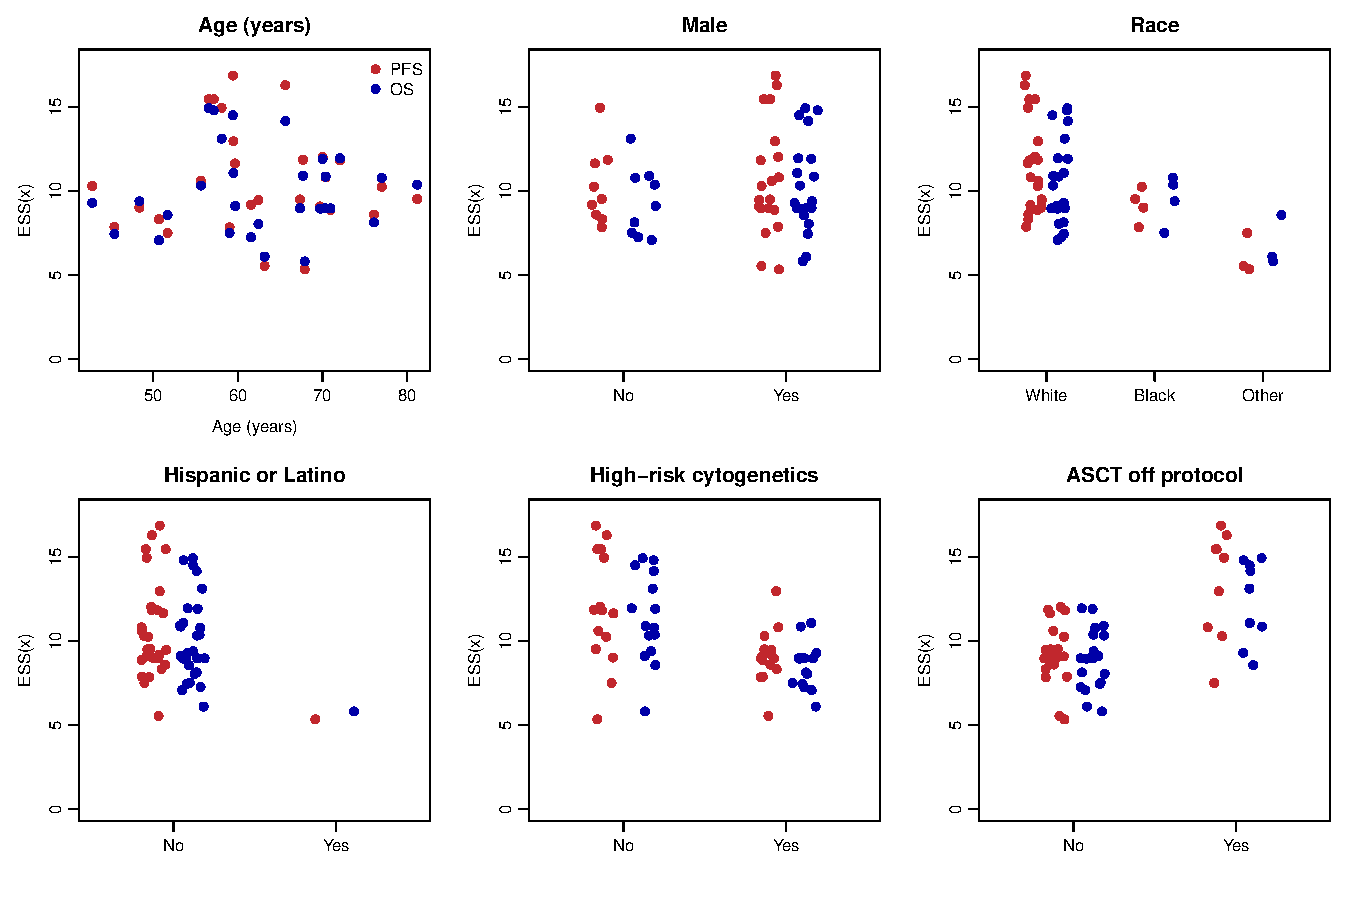
\includegraphics[width=\textwidth]{figures/fig_ess_map.pdf}
\caption{Local prior effective sample size $\mathrm{ESS}(x)=\hat\sigma_1^2/\{V_f(x)+H_g\bar\tau_0^2\}$ at the $30$ EloKRd profiles for PFS (red) and OS (blue) at $N_{\rm target}=30$, plotted against each harmonized covariate; $V_f(x)$ is the UCMM posterior variance of the log-time surface at $x$.}
\label{fig:essmap}
\end{figure}

%==============================================================================
\section{Discussion}
\label{sec:discussion}
%==============================================================================

LRC-BART combines an efficiency gain under agreement with a covariate-resolved assessment of compatibility. In the Gaussian simulations, its RMSE is about $16\%$ lower than BART-PP's under Sc1. Under global disagreement, its residual bias is about $0.04$. For a regional shift of $1.3$ residual SDs, the compatibility map and realized regional ESS distinguish the two regions, although the transition spans about one unit of the splitting covariate. The control-surface RMSE remains higher than BART-PP's, including away from the boundary. At a regional shift of two thirds of a residual SD, excessive borrowing produces bias of $0.04$ and coverage of $0.89$. The leaf calculation in Theorem~\ref{thm:map}(a) describes the dependence of detection on the spike scale and local sample size; it does not establish the performance of the full fitted ensemble.

The CAHB comparison illustrates the difficulty of kernel-local borrowing in our nonlinear ten-covariate design. It also depends on our choices for smoothing, precision scaling and joint posterior draws. We therefore interpret it as an assessment of this transfer of CAHB, with the variants reported alongside it. The survival study shows a further limitation: with $75$ controls and censoring, the median ratio can amplify control-surface bias and posterior uncertainty. We report the RMST ratio with it. In a single-arm study, trial data cannot identify a control discrepancy. The ceiling and local prior ESS then describe external support at trial profiles, but cannot demonstrate compatibility with an unobserved trial control surface.

The theoretical results condition on features that are learned in the fitted model. Map consistency requires fixed discrepancy partitions and a true discrepancy in their additive span. We have no corresponding result for the posterior over partitions. The leaf-level influence bound also treats $f$ as fixed; uncertainty in the fitted pooled surface perturbs the residuals used to estimate $g$. These limitations prevent a direct extension of the conditional results to the full posterior. The observed surface loss under Sc4 remains an empirical limitation even when profiles near the boundary are excluded.

The spike scale is global, with locality determined by the indicators. Leaf-specific scales could accommodate different degrees of compatibility, at the cost of the Inv-$\chi^2$ conjugacy. Multiple external sources would require source-specific discrepancies and a joint calibration that accounts for their information at the trial profiles; additivity of the ceilings has not been established. Binary and count outcomes require an alternative likelihood, and a nonparametric survival model would require a different RMST calculation. Prior-ESS calibration alone does not control Type I error or power. A confirmatory design would need to evaluate those operating characteristics under specified scenarios and pre-specify how the compatibility map would be used.
